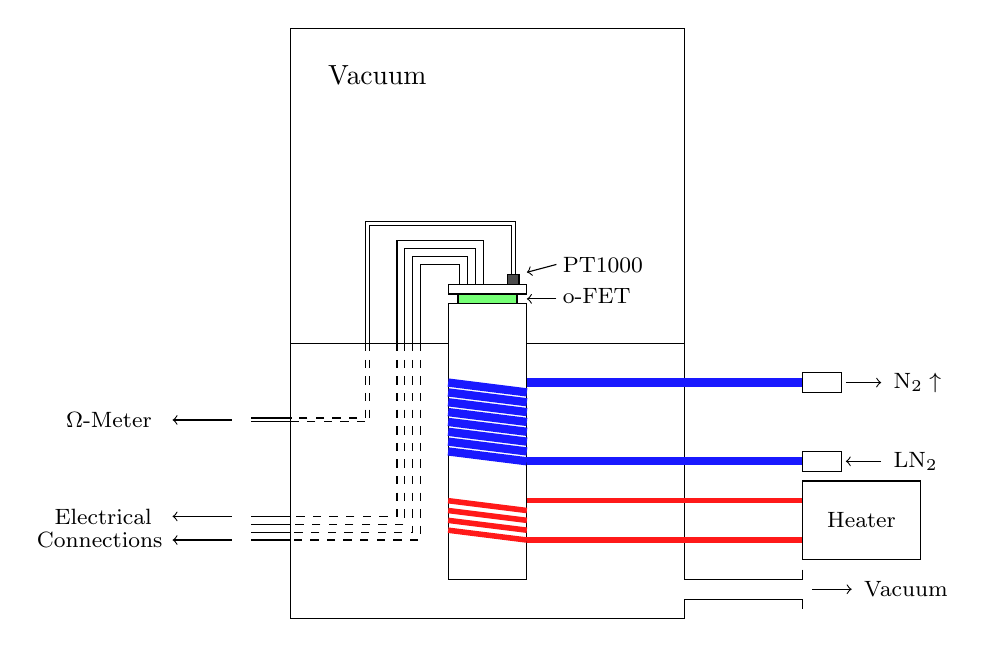
\begin{tikzpicture}[scale=0.5]

\draw [] (-1,2)--(-5,2)--(-5,-5)--(5,-5)--(5,-4.5)--(8,-4.5)--++(0,-0.25);

\draw [] (8,-3.75)--(8,-4)--(5,-4)--(5,2)--(1,2);
\draw[->] (8.25,-4.25)--++(1,0) node[right=1pt]{\footnotesize{Vacuum}};
% Solenoid core
\draw [] (-1,3)--(-1,-4)--(1,-4)--(1,3)--(-1,3);


\draw[] (8,-1.25)--(8,-0.75)--(9,-0.75)--(9,-1.25)--(8,-1.25);

\draw[] (8,1.25)--(8,0.75)--(9,.75)--(9,1.25)--(8,1.25);

\draw[->] (10,-1)--(9.1,-1);
\draw[->] (9.1,1)--(10,1);

\node at(10,1) [right=1pt]{\footnotesize{N$_2\uparrow$}};
\node at(10,-1) [right=1pt]{\footnotesize{LN$_2$}};


\draw[blue!90, line width = 3pt] (1,1)--(8,1);
\draw[blue!90, line width = 3pt] (1,-1)--(8,-1);
\draw[blue!90, line width = 3pt] (-1,1)--(1,0.75);
\draw[blue!90, line width = 3pt] (-1,0.75)--(1,0.5);
\draw[blue!90, line width = 3pt] (-1,0.5)--(1,0.25);
\draw[blue!90, line width = 3pt] (-1,0.25)--(1,0);
\draw[blue!90, line width = 3pt] (-1,0.0)--(1,-0.25);
\draw[blue!90, line width = 3pt] (-1,-0.25)--(1,-0.5);
\draw[blue!90, line width = 3pt] (-1,-0.5)--(1,-0.75);
\draw[blue!90, line width = 3pt] (-1,-0.75)--(1,-1);

\draw[red!90, line width = 2pt] (1,-2)--(8,-2);
\draw[red!90, line width = 2pt] (1,-3)--(8,-3);
\draw[red!90, line width = 2pt] (-1,-2)--(1,-2.25);
\draw[red!90, line width = 2pt] (-1,-2.25)--(1,-2.5);
\draw[red!90, line width = 2pt] (-1,-2.5)--(1,-2.75);
\draw[red!90, line width = 2pt] (-1,-2.75)--(1,-3);

\draw[] (8,-1.5)--(8,-3.5)--(11,-3.5)--(11,-1.5)--(8,-1.5);
\node at (9.5,-2.5) []{\footnotesize{Heater}};

\draw [fill = green!90, fill opacity = 0.6] (-0.75,3)--(-0.75,3.25)--(0.75,3.25)--(0.75,3)--(-0.75,3);
\node at (0.75,3.2) [right = 13pt]{\footnotesize{o-FET}};
\draw[->] (1.75,3.125)--(1,3.125);

\draw[](-0.70,3.5)--++(0,0.5)--++(-1,0)--++(0,-2);
\draw[dashed](-1.7,2)--++(0,-5)--++(-3.3,0);
\draw[](-5,-3)--(-6,-3);

\draw[](-0.5,3.5)--++(0,0.7)--++(-1.4,0)--++(0,-2.2);
\draw[dashed](-1.9,2)--++(0,-5+0.2)--++(-3.3+0.2,0);
\draw[](-5,-3+0.2)--(-6,-3+0.2);


\draw[](-0.5+0.2,3.5)--++(0,0.7+0.2)--++(-1.8,0)--++(0,-2.2-0.2);
\draw[dashed](-1.9-0.2,2)--++(0,-5+0.2+0.2)--++(-3.3+0.2+0.2,0);
\draw[](-5,-3+0.4)--(-6,-3+0.4);

\draw[](-0.5+0.2+0.2,3.5)--++(0,0.7+0.2+0.2)--++(-2.2,0)--++(0,-2.2-0.2-0.2);
\draw[dashed](-1.9-0.2-0.2,2)--++(0,-5+0.2+0.2+0.2)--++(-3.3+0.2+0.2+0.2,0);
\draw[](-5,-3+0.6)--(-6,-3+0.6);

\draw[->] (-6.5, -2.4) --(-8,-2.4) node[left=4pt]{\footnotesize{Electrical}};
\draw[->] (-6.5, -3) --(-8,-3) node[left=0.1pt]{\footnotesize{Connections}};


\draw [] (-1,3.25)--(-1,3.5)--(1,3.5)--(1,3.25)--(-1,3.25);
\draw [fill = black!70] (0.5,3.5)--(0.5,3.75)--(0.8,3.75)--(0.8,3.5)--(0.5,3.5);
\draw[] (0.6,3.75)--(0.6,5)--(-3,5)--(-3,2);
\draw[dashed] (-3,2)--(-3,0)--(-5,0);
\draw[](-5,0)--++(-1,0);


\draw[] (0.7,3.75)--(0.7,5.1)--(-3.1,5.1)--(-3.1,2);
\draw[dashed] (-3.1,2)--(-3.1,0.1)--(-5,0.1);
\draw[](-5,0.1)--++(-1,0);
\draw[->] (-6.5, 0.05) --++(-1.5,0) node[left=4pt]{\footnotesize{$\Omega$-Meter}};


\draw [] (-5,2)--(-5,10)--(5,10)--(5,2);

\node at (-5,10) [below right = 10pt]{Vacuum};

\node at (0.75,4.0) [right = 13pt]{\footnotesize{PT1000}};
\draw[->] (1.75,4.0)--(1.0,3.8);

\end{tikzpicture}